\documentclass[10pt,a4paper]{scrartcl}
\PassOptionsToPackage{table}{xcolor}
\usepackage[utf8]{inputenc}
\usepackage[T1]{fontenc}
\usepackage[ngerman]{babel}
\usepackage{microtype, multicol, marginnote, bera, parskip}
\usepackage{listings, amsmath, amssymb, graphicx, tikz, epic}
\usepackage{stmaryrd} %for lightning arrow
\usepackage{pstricks, pst-node, pst-tree, pdflscape}
\usepackage[babel=true]{csquotes}
\usepackage{placeins}
\tolerance=2000
\setcounter{secnumdepth}{0}
\usepackage[inner=2cm,outer=2cm,top=1.5cm,bottom=1.5cm,includeheadfoot]{geometry}
\usepackage{multirow}
\newcommand{\subExercise}[1]{\vspace{0.5em} \noindent{\bf #1)}}
\author{Michael Mardaus \and Andrey Tyukin}
\title{
\includegraphics[scale=0.2]{../logo_schriftzug}\\
Technische Informatik: Abgabe 4}

\begin{document}

\maketitle

\section*{Exercise 4.1 (Full adder from decoder)}

\vspace{1em}
\begin{figure}[h]
  \centering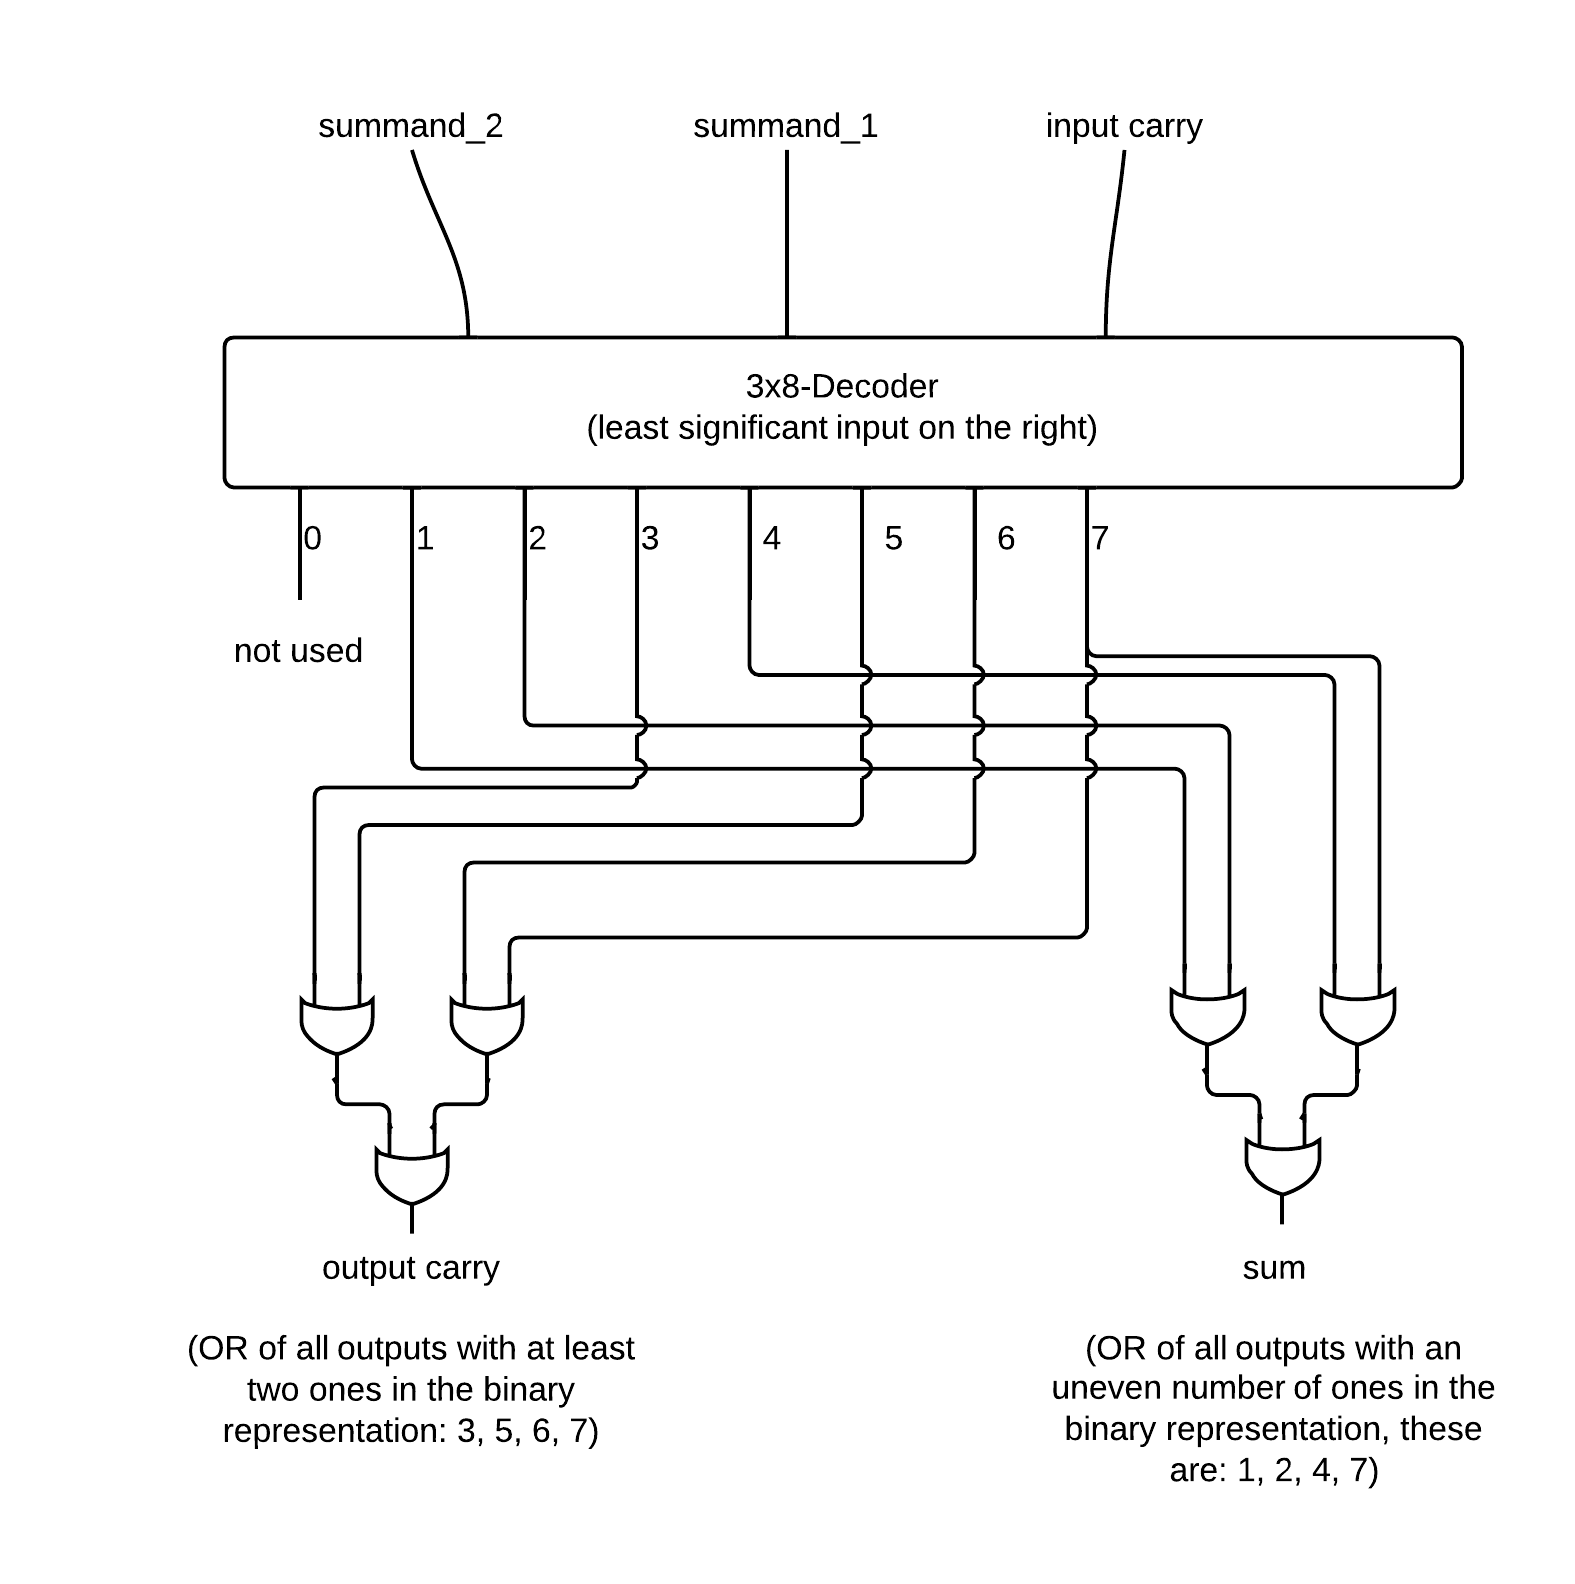
\includegraphics[width=0.6\linewidth]{images/fullAdder.png}
\end{figure}
\vspace{1em}

\FloatBarrier
\newpage
\section*{Exercise 4.2 (Subtractors)}
\subExercise{a}
Here are the tables for the two circuits we wish to implement 
(namely Half-Subtractor and Full-Subtractor):

\vspace{0.5em}
\begin{tabular}{|c c|c c|}
  \hline
  minuend & subtrahend & underflow & difference \\
  \hline
  0 & 0 & 0 & 0 \\
  0 & 1 & 1 & 1 \\
  1 & 0 & 0 & 1 \\
  1 & 1 & 0 & 0 \\
  \hline
\end{tabular}

If we read $ms$ as numbers with high order bit on the left: 
\begin{align*}
  u_{out} &= m_1 \\
  d &= m_1 + m_2.
\end{align*}

\vspace{0.5em}
\begin{tabular}{|c c c|c c|}
  \hline
  minuend & subtrahend & underflow & underflow & difference \\
  \hline
  0 & 0 & 0 & 0 & 0 \\
  0 & 0 & 1 & 1 & 1 \\ 
  0 & 1 & 0 & 1 & 1 \\ 
  0 & 1 & 1 & 1 & 0 \\ 
  1 & 0 & 0 & 0 & 1 \\ 
  1 & 0 & 1 & 0 & 0 \\ 
  1 & 1 & 0 & 0 & 0 \\ 
  1 & 1 & 1 & 1 & 1 \\ 
  \hline
\end{tabular}

Again, in SOP-notation with high-order bit on the left:
\begin{align*}
  u_{out} &= m_1 + m_2 + m_3 + m_7 \\
  d &= m_1 + m_2 + m_4 + m_7.
\end{align*}

\subExercise{b} 
More or less compact symbolic representations 
of these two circuits are as follows 
(first component is always the resulting underflow, 
 second is the actual difference):
\[
  HalfSubtractor(m,s) = (\bar m s, m \not\leftrightarrow s)
\]
\[
  FullSubtractor(m,s,u) = 
    (\bar m \not\leftrightarrow su, 
     m \not\leftrightarrow s \not\leftrightarrow u
    )
\]

\subExercise{c} 
Now we want to simplify both components (difference and undeflow) 
of the full subtractor using Karnaugh diagrams. We begin with the
difference:

\vspace{0.5em}
\begin{tabular}{|c c|c c c c|}
  \hline 
    & & \multicolumn{4}{c|}{minuend / subtrahend} \\
    & & 00 & 01 & 11 & 10 \\
  \hline
    \multirow{2}{*}{underflow} & 0 &   & \cellcolor{blue}1 &   & \cellcolor{orange}1 \\
                               & 1 & \cellcolor{red}1 &   & \cellcolor{green}1 &   \\
  \hline
\end{tabular}

It seems that this diagram is not simplifiable at all: we have to cover every
one by an own 1x1 block. The simpliest expression for difference is thus:
\[
  d = \bar m \bar s u + \bar m s \bar u + m s u + m \bar s \bar u
\]

The ones for the output-underflow can be covered by
three 2x1 blocks, which all intersect at 011 (we use additive color combination,
light gray is supposed to be combination of red, green and blue):
\vspace{0.5em}
\begin{tabular}{|c c|c c c c|}
  \hline 
    & & \multicolumn{4}{c|}{minuend / subtrahend} \\
    & & 00 & 01 & 11 & 10 \\
  \hline
    \multirow{2}{*}{underflow} & 0 & 0 & \cellcolor{green}{1} & 0 & 0 \\
                               & 1 & \cellcolor{red}{1} & \cellcolor{lightgray}{1} & \cellcolor{blue}{1} & 0 \\
  \hline
\end{tabular}

Thus, the simplified formula for the output-underflow is:
\[
u_{out} = \bar m u + \bar m s + su.
\]

\subExercise{d}

\vspace{1em}
\begin{figure}[h]
  \centering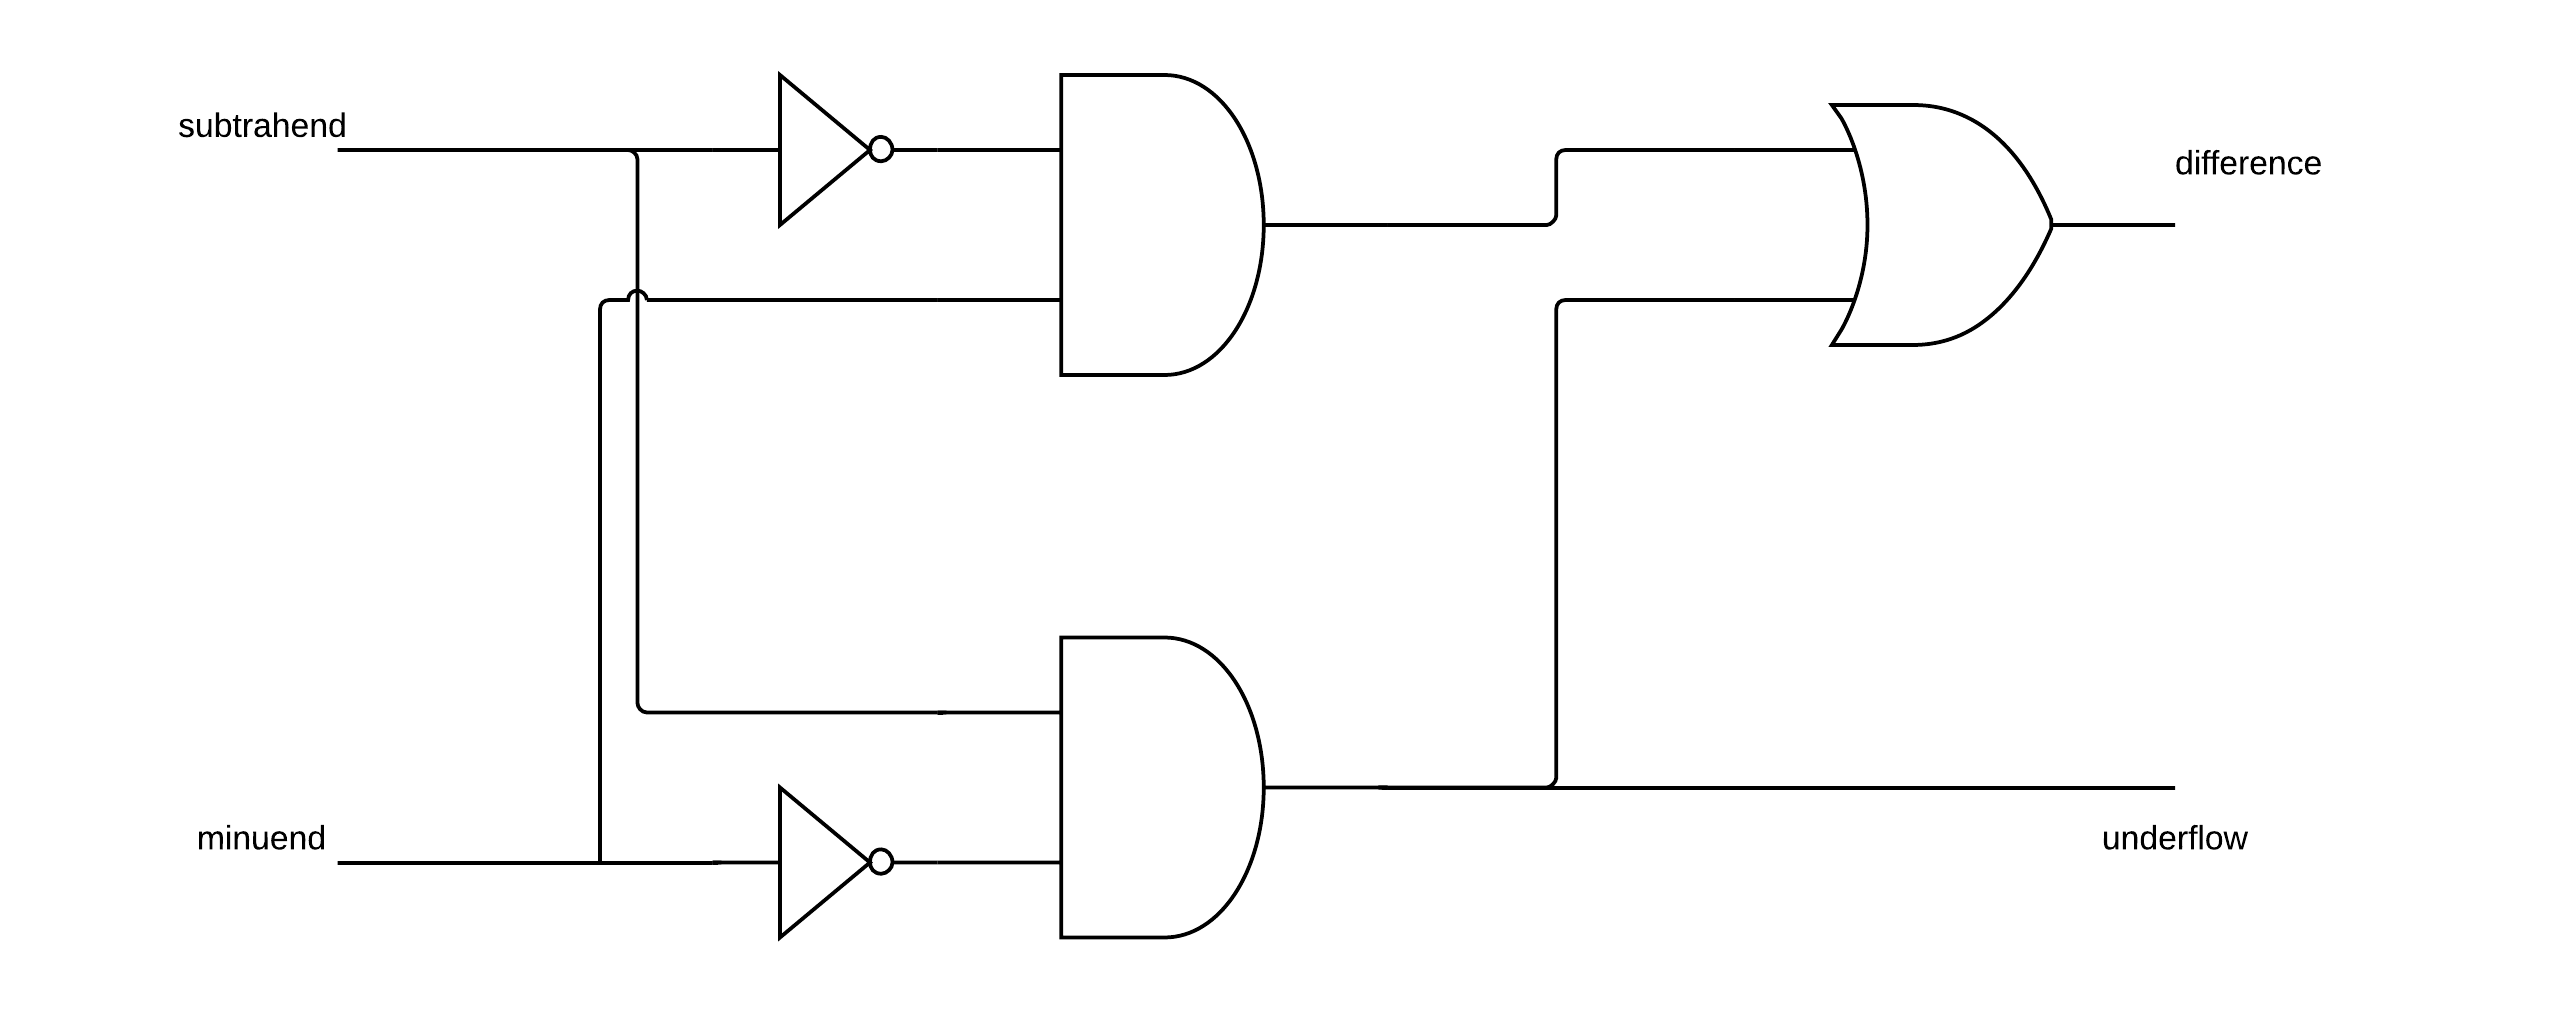
\includegraphics[width=0.75\linewidth]{images/halfSubtractor.png}
  \caption{Half subtractor.}
\end{figure}
\vspace{1em}

\vspace{1em}
\begin{figure}[h]
  \centering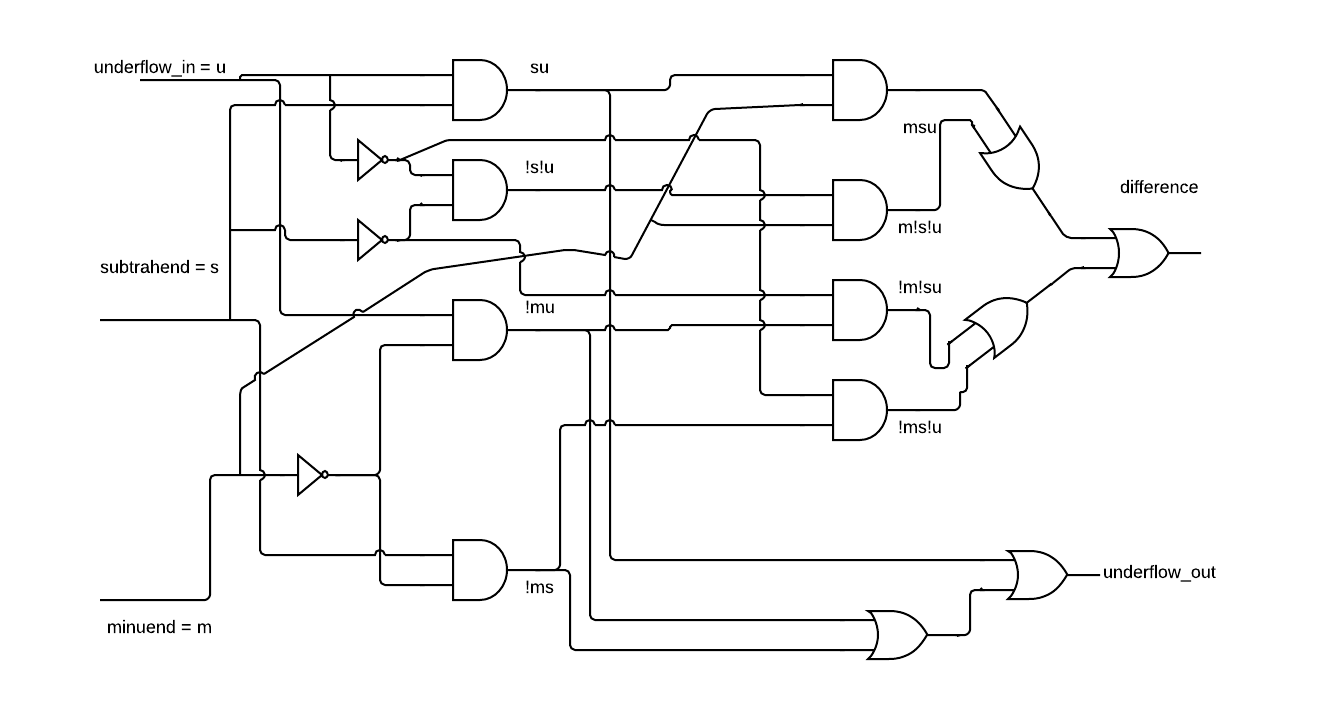
\includegraphics[width=0.75\linewidth]{images/fullSubtractor.png}
  \caption{Full subtractor. We recycled as many gatters as we could for both sub-circuits. Reason: that's the maximal complexity allowed for free LucidChart accounts...}
\end{figure}
\vspace{1em}

\FloatBarrier
\section*{Exercise 4.3 (Betting and Racing)}

\begin{tabular}{|l||l|l|l|l||l||l|l|}\hline
i & $x_1$ & $x_2$ & $x_3$ & $x_4$ & $f_1$ & $f_{2a}$ & $f_{2b}$ \\\hline\hline
0 & 0 & 0 & 0 & 0 &                 &   &    \\\hline
1 & 0 & 0 & 0 & 1 &                 &   &    \\\hline
2 & 0 & 0 & 1 & 0 &    1 ($B_2$)    &   &    \\\hline
3 & 0 & 0 & 1 & 1 &    1 ($B_3$)    & 1 & 1  \\\hline
4 & 0 & 1 & 0 & 0 &                 &   &    \\\hline
5 & 0 & 1 & 0 & 1 &    1 ($B_3$)    & 1 & 1  \\\hline
6 & 0 & 1 & 1 & 0 &                 &   &    \\\hline
7 & 0 & 1 & 1 & 1 &                 & 1 & 1  \\\hline
8 & 1 & 0 & 0 & 0 &    1 ($B_1$)    &   &    \\\hline
9 & 1 & 0 & 0 & 1 &    0 ($B_1+B_3$)&   &    \\\hline
10 & 1 & 0 & 1 & 0 &   1 ($B_1$)    &   & D  \\\hline
11 & 1 & 0 & 1 & 1 &   1 ($B_1$)    &   & D  \\\hline
12 & 1 & 1 & 0 & 0 &                &   & D  \\\hline
13 & 1 & 1 & 0 & 1 &                &   & D  \\\hline
14 & 1 & 1 & 1 & 0 &                &   & D  \\\hline
15 & 1 & 1 & 1 & 1 &                & 1 & D  \\\hline
\end{tabular}

\subExercise{a1}
$f_1 = 1 \Leftrightarrow B_1 . \neg B_2 . \neg B_3 + \neg B_1 . B_2 . \neg B_3 + \neg B_1 . \neg B_2 . B_3$ \\ where
\begin{itemize}
 \item $B_1 = 1 \Leftrightarrow x_1 . \neg x_2 = 1$ 
 \item $B_2 = 1 \Leftrightarrow \neg x_1 . \neg x_2 . x_3 . \neg x_4  = 1$
 \item $B_3 = 1 \Leftrightarrow x_4 . \text{only one of}(x_1,x_2,x_3) = 1$
\end{itemize}
brings us to column $f_1$ in the table above and leeds to the Karnaugh table:

\begin{tabular}{|c||c|c|c|c|}
  \hline 
            & \multicolumn{4}{c|}{$x_3x_4$} \\
$x_1x_2$ & 00                  & 01                  & 11                 & 10                \\ \hline
    00   &                     & \cellcolor{yellow}1 & \cellcolor{green}1 &                   \\ \hline
    01   &                     & \cellcolor{red}1    &                    &                   \\ \hline
    11   &                     &                     &                    &                   \\ \hline
    10   & \cellcolor{orange}1 &                     & \cellcolor{blue}1  & \cellcolor{blue}1 \\
  \hline
\end{tabular}
which yields: $f_1 =  \textcolor{blue}{x_1\neg x_2x_3}+
                      \textcolor{red}{\neg x_1\neg x_3x_4}+
                      \textcolor{green}{\neg x_1\neg x_2x_4}+
                      \textcolor{orange}{x_1\neg x_2\neg x_3\neg x_4}$

                      
                      
\subExercise{a2}
$f_{2a} = 1 \Leftrightarrow (x_1x_2x_3x_4)_2 | 1101001 ($in decimal $105=3\times5\times7)$\\
brings us to column $f_{2a}$ in the table above and leeds to the Karnaugh table:\\
\begin{tabular}{|c||c|c|c|c|}
  \hline 
            & \multicolumn{4}{c|}{$x_3x_4$} \\
$x_1x_2$ & 00                  & 01                  & 11                 & 10                \\ \hline
    00   &                     &                     & \cellcolor{green}1 &                   \\ \hline
    01   &                     & \cellcolor{red}1    & \cellcolor{gray}1  &                   \\ \hline
    11   &                     &                     & \cellcolor{blue}1  &                   \\ \hline
    10   &                     &                     &                    &                   \\
  \hline
\end{tabular}
which yields $f_{2a} = \textcolor{red}{\neg x_1x_2x_4}+
                       \textcolor{green}{\neg x_1x_3x_4}+
                       \textcolor{blue}{x_2x_3x_4}$

                 
                 
\subExercise{b}


$f_{2b} = 1 \Leftrightarrow 0000\leq(x_1x_2x_3x_4)_2\leq1001 | 1101001 $ gives column $f_{2b}$ in the table above, Karnaugh table:\\
\begin{tabular}{|c||c|c|c|c|}
  \hline 
            & \multicolumn{4}{c|}{$x_3x_4$} \\
$x_1x_2$ & 00                  & 01                  & 11                 & 10                \\ \hline
    00   &                     &                     & \cellcolor{green}1 &                   \\ \hline
    01   &                     & \cellcolor{red}1    & \cellcolor{yellow}1&                   \\ \hline
    11   & D                   & \cellcolor{red}D    & \cellcolor{red}D   & D                 \\ \hline
    10   &                     &                     & D                  & D                 \\
  \hline
\end{tabular}
which yields $f_{2b} = \textcolor{red}{x_2x_4}+\textcolor{green}{\neg x_1x_3x_4}$


\end{document}
